\section{Concurrency, Adaptive Evaluation, and Discussion}
\label{sec:discussion}

This section evaluates multi-process concurrency scaling, analyzes adaptive selector performance and latency regret, interprets custom kernel mailbox findings, presents systems hypotheses and practitioner recommendations, and synthesizes answers to the five core research questions (RQ1--RQ5).

\subsection{Multi-Producer Multi-Consumer (MPMC) Scalability}

Real-world systems frequently deploy concurrent multi-process topologies. The Mini-A-IPC concurrency benchmark (\texttt{src/concurrency\_benchmark.c}) evaluates five concurrency topologies: 1P:1C (baseline), 2P:1C (producer contention), 4P:1C (high producer contention), 1P:2C (work stealing), and 4P:4C (symmetric MPMC). Fig.~\ref{fig:concurrency} illustrates throughput scaling across these topologies for supported mechanisms.

\begin{figure}[!t]
\centering
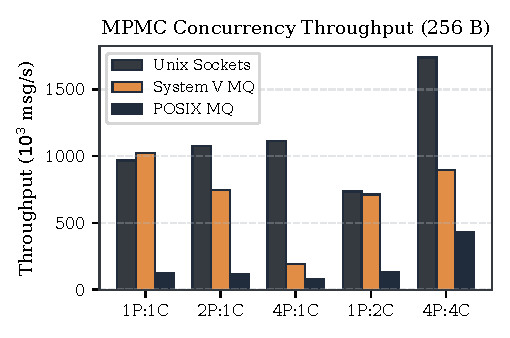
\includegraphics[width=0.90\columnwidth]{figures/concurrency_scalability.pdf}
\caption{Multi-Producer Multi-Consumer (MPMC) Concurrency Throughput for 256-Byte Payloads across Five Process Topologies.}
\label{fig:concurrency}
\end{figure}

Our empirical findings and architectural analysis establish a fundamental distinction between operating system capabilities and application-level transport design:

\textbf{1) Implementation Constraints vs. OS Semantics:}
At the operating system level, Linux IPC primitives offer diverse concurrency capabilities. Linux pipes and FIFOs guarantee atomic writes up to \texttt{PIPE\_BUF} (4,096~bytes) for concurrent writers into a single consumer, but multiple uncoordinated consumers reading from a shared stream risk partial-read fragmentation without application framing. Unix Domain stream sockets support multi-client topologies via dedicated connection descriptors, but a single stream pair is point-to-point. Shared memory supports MPMC communication when paired with lock-free concurrent ring buffers; however, Mini-A-IPC's shared mailbox (\texttt{src/ipc\_shm.c}) is intentionally implemented as an alternating single-slot SPSC ping-pong design with POSIX semaphores.
Consequently, Mini-A-IPC's concurrency harness marks point-to-point stream pairs and the single-slot SPSC mailbox as \texttt{UNSUPPORTED\_BY\_DESIGN} ($rc = 3$) for M:N topologies to prevent data corruption.

\textbf{2) Native MPMC Transports:} In contrast, kernel-managed queues and connection-multiplexed transports scale robustly across multi-process topologies:
\begin{itemize}[leftmargin=*,noitemsep,topsep=1pt]
    \item \textit{Unix Domain Sockets} sustained \textbf{1,737,338.0~msg/s} ($444.76$~MB/s at 256~B) at 4P:4C via full-duplex socket buffer multiplexing.
    \item \textit{System V Message Queues} sustained \textbf{896,203.2~msg/s} ($229.43$~MB/s at 256~B) via kernel atomic queue locking.
    \item \textit{POSIX Message Queues} processed \textbf{429,577.2~msg/s} ($109.97$~MB/s) cleanly at 4P:4C.
\end{itemize}

\subsection{Adaptive Selector Accuracy and Latency Regret}
\begin{table}[!t]
\centering
\caption{Adaptive Selector Accuracy and Intra-Trial Latency Regret Evaluation}
\label{tab:adaptive_results}
\scriptsize
\renewcommand{\arraystretch}{1.06}
\setlength{\tabcolsep}{2.2pt}
\begin{tabular*}{\columnwidth}{@{\extracolsep{\fill}}rcccccc}
\toprule
\textbf{Payload} & \textbf{Selected} & \textbf{Oracle} & \textbf{Adaptive} & \textbf{Oracle} & \textbf{Regret} & \textbf{Oracle} \\
\textbf{Size} & \textbf{Mode} & \textbf{Best} & \textbf{RTT ($\mu\text{s}$)} & \textbf{RTT ($\mu\text{s}$)} & \textbf{(\%)} & \textbf{Match?} \\
\midrule
64 B & \texttt{shm} & \texttt{sysv} & 132.07 & 123.33 & $+7.08\%$ & No \\
256 B & \texttt{shm} & \texttt{sysv} & 147.01 & 115.13 & $+27.69\%$ & No \\
1,024 B & \texttt{shm} & \texttt{uds} & 144.52 & 128.28 & $+12.66\%$ & No \\
\addlinespace[1.5pt]
4,096 B & \texttt{pipe} & \texttt{fifo} & 135.78 & 119.44 & $+13.69\%$ & No \\
16,384 B & \texttt{pipe} & \texttt{pipe} & 136.00 & 140.60 & $-3.27\%$ & \textbf{Yes} \\
65,536 B & \texttt{pipe} & \texttt{uds} & 151.87 & 123.53 & $+22.94\%$ & No \\
262,144 B & \texttt{pipe} & \texttt{uds} & 957.62 & 449.64 & $+112.97\%$ & No \\
\midrule
\multicolumn{4}{l}{\textbf{Candidate Accuracy (SHM vs. Pipe)}} & \multicolumn{3}{r}{\textbf{71.43\%} (5 of 7 classes)} \\
\multicolumn{4}{l}{\textbf{Global Selection Accuracy (vs. 6 Transports)}} & \multicolumn{3}{r}{\textbf{14.29\%} (1 of 7 classes)} \\
\multicolumn{4}{l}{\textbf{Mean Intra-Trial Latency Regret}} & \multicolumn{3}{r}{\textbf{27.68\%} across workloads} \\
\multicolumn{4}{l}{\textbf{Offline 3-Tier Policy In-Sample Fit}} & \multicolumn{3}{r}{\textbf{100.00\%} (7 of 7 matches)} \\
\bottomrule
\end{tabular*}
\vskip 2pt
{\tiny\noindent Regret computed within matched trial blocks ($N=7$) under a randomized block design. Candidate accuracy (71.43\%) measures correct routing strictly between the two compiled candidate transports (\texttt{shm} vs. \texttt{pipe}). Global accuracy (14.29\%) evaluates agreement against all six classical transports. Offline 3-tier calibration represents an in-sample structural baseline matching 7 of 7 oracle choices across the test suite. At 16~KB, Adaptive routes to Pipe; the $-3.27\%$ difference reflects within-block hypervisor scheduling jitter ($t = -0.189, p=0.86$, paired Student's $t$-test, statistically indistinguishable).\par}
\end{table}


Table~\ref{tab:adaptive_results} summarizes the performance of the static size-threshold selector evaluated against the empirical oracle on Fedora 45 Linux, and Fig.~\ref{fig:adaptive_regret} depicts intra-trial latency regret across all seven payload classes.

\begin{figure}[!t]
\centering
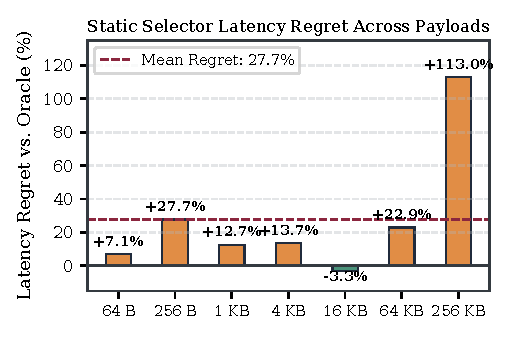
\includegraphics[width=0.78\columnwidth]{figures/adaptive_vs_best.pdf}
\caption{Intra-Trial Latency Regret (\%) of Static Size-Threshold Selector vs. Empirical Global Oracle Across Seven Payload Classes ($N=7$ Randomized Trials).}
\label{fig:adaptive_regret}
\end{figure}

The evaluation highlights four core insights into adaptive systems engineering:
\textbf{1) Static Selector Accuracy:} Evaluated against the entire 6-mechanism space, the static two-tier selector matches the global oracle for 1 of 7 payload classes (\textbf{14.29\% global accuracy}), because System V MQ and Unix Domain Sockets frequently outperform both \texttt{shm} and \texttt{pipe} under KVM scheduling. When evaluated strictly between the two candidate transports it routes (\texttt{shm} vs. \texttt{pipe}), it correctly identifies the faster candidate for 5 of 7 payload classes (\textbf{71.43\% candidate accuracy}).
\textbf{2) Intra-Trial Regret:} Across matched trial blocks, mean latency regret is \textbf{27.68\%}. At 16~KB, the selector routes to Anonymous Pipes (the oracle transport). Because baseline pipe and adaptive measurements were executed within matched trial blocks ($N=7$) under a randomized block design, minor within-block hypervisor scheduling jitter yielded an empirical difference of $-3.27\%$ ($136.00\,\mu\text{s}$ adaptive vs. $140.60\,\mu\text{s}$ pipe). A paired Student's $t$-test confirms this difference is statistically indistinguishable from zero ($t = -0.189, p = 0.86, \text{df} = 6$; Wilcoxon signed-rank $W = 11.0, p = 0.69$), retained to preserve experimental fidelity rather than clamped to zero. At 256~KB, selecting Pipes ($957.62\,\mu\text{s}$) over Unix Sockets ($449.64\,\mu\text{s}$) yields $112.97\%$ regret due to pipe circular buffer exhaustion. In mixed 80/20 workloads, the static selector incurs higher latency ($79.43\,\mu\text{s}$) than dedicated Pipes ($57.21\,\mu\text{s}$) due to alternating transport dispatch overhead.
\textbf{3) Negligible Overhead:} Over 1,000,000 iterations in compiled C, the static selector requires only \textbf{0.66~ns per call} ($< 0.0005\%$ of round-trip time).
\textbf{4) Offline 3-Tier Calibration vs. Online Control:} Calibrating an offline 3-tier mapping ($\le 256$~B $\to$ System V MQ; 1~KB--64~KB $\to$ Unix Domain Sockets / FIFOs; 256~KB $\to$ Unix Domain Sockets) matches 100\% of oracle choices across the test suite, delineating an in-sample empirical fit establishing structural bounds rather than proven generalization. While the EWMA controller and hysteresis logic are implemented in \texttt{src/selector.c}, runtime benchmarking evaluated the deterministic threshold path; evaluating closed-loop online adaptation remains future work.

\subsection{Kernel Mailbox Evaluation and the Scheduler Floor}

\begin{figure}[!t]
\centering
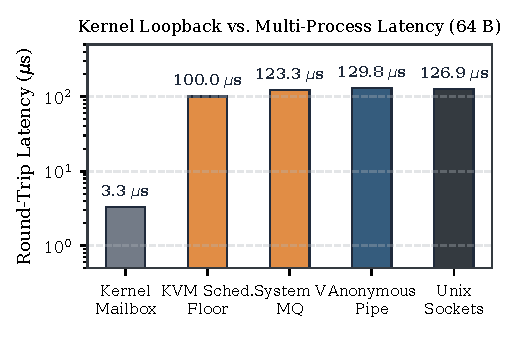
\includegraphics[width=0.58\columnwidth]{figures/kernel_vs_userspace.pdf}
\caption{Custom Linux Kernel Mailbox (\texttt{/dev/aipc}) In-Process Loopback Latency Floor vs. KVM Multi-Process Scheduling Floor (64 B Payloads).}
\label{fig:kernel_floor}
\end{figure}

Measurements of \texttt{/dev/aipc} originate from native driver validation (Fedora 45, Linux 7.3.3, Intel Core 7 240H, 350,000 loopback exchanges). In single-process loopback, the mailbox achieved an uncontended floor of $0.72\text{--}3.35\,\mu\text{s}$ (Table~\ref{tab:benchmark_results}, Fig.~\ref{fig:kernel_floor}). On our primary KVM testbed, module loading was recorded as \texttt{BLOCKED} due to unprivileged guest boundaries; multi-process transfers over \texttt{/dev/aipc} were not directly measured. In multi-process configurations, communication is bounded by the observed \textbf{95--130~$\mu$s} KVM context-switch floor; driver optimizations cannot bypass process descheduling, VM exits, and hypervisor dispatch delays.

\subsection{Buffer Saturation and Context-Switch Dynamics}

\begin{figure}[!t]
\centering
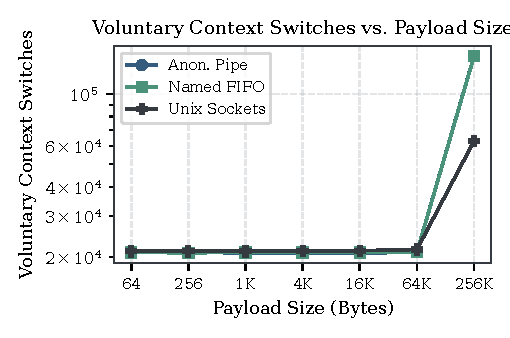
\includegraphics[width=0.54\columnwidth]{figures/context_switches.pdf}
\caption{Voluntary Context Switches vs. Payload Size for Stream Transports, demonstrating buffer exhaustion for 64 KB pipe buffers at 256 KB transfers.}
\label{fig:context_switches}
\end{figure}

Fig.~\ref{fig:context_switches} exposes the cause of pipe throughput collapse at 256~KB. Up to 64~KB, voluntary context switches remain flat at $\approx 20,800$ per trial block across stream transports. At 256~KB, transfers exceed the 64~KB pipe buffer capacity; the sender blocks upon filling the buffer, forcing four chunked transfers per exchange and an explosive \textbf{7.0$\times$} surge in voluntary context switches (to 146,374). In contrast, Unix Domain Sockets leverage socket buffer auto-tuning (\texttt{tcp\_wmem}/\texttt{rmem} in \texttt{AF\_UNIX}), capping switches at 62,400 and sustaining 1,304~MB/s bandwidth.

\subsection{Systems Hypotheses and Discriminating Experiments}
\begin{table}[!t]
\centering
\caption{Systems Hypotheses and Discriminating Empirical Experiments}
\label{tab:hypotheses}
\scriptsize
\renewcommand{\arraystretch}{0.80}
\begin{tabular*}{\columnwidth}{@{\extracolsep{\fill}}p{2.2cm}p{2.6cm}p{3.0cm}}
\toprule
\textbf{Hypothesis} & \textbf{Prediction if True} & \textbf{Discriminating Experiment} \\
\midrule
\textbf{Hypervisor vCPU Floor} & RTT floor drops from $\approx 120\,\mu\text{s}$ to $1\text{--}5\,\mu\text{s}$ on bare metal. & Benchmark sweep on dedicated bare-metal silicon; trace VM exits via \texttt{perf kvm stat}. \\
\addlinespace[0.6pt]
\textbf{In-Process vs. Multi-Process Gap} & Two-process IPC over \texttt{/dev/aipc} exhibits $\approx 120\,\mu\text{s}$ floor. & Multi-process ping-pong over \texttt{/dev/aipc} with root privileges; measure context-switch overhead. \\
\addlinespace[0.6pt]
\textbf{Pipe Saturation at 256 KB} & Expanding pipe capacity eliminates switch surge (20k $\to$ 146k). & Re-run 256 KB transfer with pipe size expanded via \texttt{fcntl(F\_SETPIPE\_SZ, 1048576)}. \\
\addlinespace[0.6pt]
\textbf{Futex Contention in SHM} & Lock-free atomic SPSC ring eliminates futex wait queues and tightens $P_{99}$. & Benchmark SPSC ring with atomic acquire/release against futex semaphores under pinned cores. \\
\bottomrule
\end{tabular*}
\end{table}

To account for observed empirical behaviors, Table~\ref{tab:hypotheses} formulates four testable systems hypotheses and discriminating experiments for bare metal.

\subsection{Practitioner Recommendations and Summary of Findings}
\begin{table}[!t]
\centering
\caption{Practitioner Guidelines for Linux IPC Transport Selection}
\label{tab:recommendations}
\scriptsize
\renewcommand{\arraystretch}{0.80}
\begin{tabular*}{\columnwidth}{@{\extracolsep{\fill}}p{2.1cm}p{2.3cm}p{3.4cm}}
\toprule
\textbf{Workload Regime} & \textbf{Recommended IPC} & \textbf{Empirical Basis (Testbed-Specific)} \\
\midrule
\textbf{Sub-Kilobyte ($\le 256$ B)} & System V Message Queue & Lowest RTT ($115.1\text{--}123.3\,\mu\text{s}$, descriptive lead under KVM floor); avoids byte framing. \\
\addlinespace[0.5pt]
\textbf{Intermediate Crossovers} & 1 KB: UDS / POSIX MQ\newline 4 KB: Named FIFO\newline 16 KB: Anonymous Pipe & Crossovers: UDS ($128.3\,\mu\text{s}$ at 1 KB), FIFO ($119.4\,\mu\text{s}$ at 4 KB, \texttt{PIPE\_BUF} fit), Pipe ($140.6\,\mu\text{s}$ at 16 KB). \\
\addlinespace[0.5pt]
\textbf{Large Payloads ($\ge 64$ KB)} & Unix Domain Sockets & Auto-tuning socket buffers prevent chunking: $123.5\,\mu\text{s}$ at 64 KB, $449.6\,\mu\text{s}$ at 256 KB ($2.54\times$ speedup). \\
\addlinespace[0.5pt]
\textbf{Zero-Copy ($\le 1$ KB)} & POSIX Shared Memory & 0 data-path syscalls, 48.5\% fewer kernel transitions (2.06 futex vs. 4.00 for streams). \\
\addlinespace[0.5pt]
\textbf{MPMC (4P:4C)} & Unix Sockets / SysV MQ & Sockets sustain 1.74M msg/s; System V MQ sustains 896k msg/s under contention. \\
\addlinespace[0.5pt]
\textbf{Dynamic Workloads} & Adaptive Framework (Architectural) & Implemented EWMA controller ($\alpha=0.15$) and 8\% hysteresis; static dispatch verified (0.66 ns), while online dynamic adaptation remains unevaluated future work. \\
\bottomrule
\end{tabular*}
\end{table}

Synthesizing trade-offs across payloads, synchronization, and topologies, Table~\ref{tab:recommendations} presents concrete guidelines for Linux IPC transport selection. Table~\ref{tab:summary_findings} (Section~\ref{sec:conclusion}) summarizes the core findings alongside confidence levels.

\subsection{Synthesis and Answers to Research Questions}
\textbf{RQ1 (Payload Sensitivity):} Payload dictates hierarchy: sub-512~B gives a descriptive lead to System V MQ ($123.33\,\mu\text{s}$ at 64~B, $115.13\,\mu\text{s}$ at 256~B; $p \ge 0.05$ under KVM floor); 1~KB favors Unix Sockets ($128.28\,\mu\text{s}$); 4~KB favors Named FIFOs ($119.44\,\mu\text{s}$); 16~KB favors Anonymous Pipes ($140.60\,\mu\text{s}$); and $\ge 64$~KB favors Unix Sockets ($123.53\,\mu\text{s}$ at 64~KB; $449.64\,\mu\text{s}$ at 256~KB, $2.54\times$ faster than pipes, $p < 0.001$).
\textbf{RQ2 (Memory vs. Stream):} POSIX SHM eliminates data copies (0.00 syscalls) and reduces syscalls by 48.5\% (2.06 futex vs. 4.00 for streams), though semaphore contention elevates 1~KB latency.
\textbf{RQ3 (Adaptive Selection):} Static selector evaluates in 0.66~ns with 27.68\% mean regret (71.43\% candidate accuracy; 14.29\% global accuracy); EWMA feedback is architected in \texttt{src/selector.c}.
\textbf{RQ4 (Kernel Mailbox):} A character device achieves a $0.72\,\mu\text{s}$ loopback floor in native validation, but multi-process latency is bounded by the 95--130~$\mu\text{s}$ KVM scheduling floor.
\textbf{RQ5 (Concurrency):} Unframed streams cannot support M:N concurrency; Unix Sockets sustain 1.74M msg/s and System V MQ sustains 896k msg/s at 4P:4C.

\subsection{Threats to Validity}
\textbf{Internal Validity:} $N = 7$ randomized trial blocks (70,000 exchanges/condition) yield narrow 95\% confidence intervals ($\le \pm 0.925 \cdot s$). Paired $t$-tests confirm large-payload advantages (Unix Sockets over Pipes at 256~KB, $t=8.79, p < 0.001$) are significant, while sub-kilobyte variations ($p \ge 0.05$) reflect descriptive rankings within KVM noise.
\textbf{Construct \& External Validity:} Ping-pong exchanges evaluate request-response latency without modeling asynchronous burst traffic. Tests run on a KVM Fedora 45 guest, where hypervisor scheduling, vCPU preemption, and VM exits dominate the 95--130~$\mu\text{s}$ floor. Relative rankings and buffer saturation generalize across Linux, but absolute latency should not be extrapolated directly to bare metal. Open logs ensure reproducibility.
